\section{Problema 2: La centralita (de gas)}

\subsection{Presentaci\'on del problema}
En una regi\'on del pa\'is se est\'a considerando realizar una inversi\'on fuerte para proveer de gas natural
a un conjunto de pueblos que no disponen a\'un de este recurso. Para ello, es posible ubicar centrales
distribuidoras de gas en algunos de los pueblos y construir tuber\'ias para distribuir el gas de un pueblo a
otro. Un pueblo ser\'a provisto de gas siempre que exista alg\'un camino por medio de tuber\'ia hasta alguna
de las centrales (incluso si este camino pasa por otros pueblos). Debido al elevado costo de construcci\'on
de las centrales distribuidoras, el presupuesto con el que se cuenta alcanza para construir a lo sumo k
centrales.

Por otro lado, los ingenieros a cargo de este proyecto saben que mientras m\'as larga sea una tuber\'ia
construida entre dos pueblos, mayor es el riesgo de roturas y escapes de gas durante el trayecto (la
longitud de una tuber\'ia que conecta dos pueblos est\'a dada por la distancia entre estos dos pueblos).
En este sentido, se defini\'o el riesgo asociado a cada posible plan de construcci\'on como la mayor de las
longitudes de las tuber\'ias construidas en dicho plan.

Se pide escribir un algoritmo que determine un plan de construcci\'on de tuber\'ias y centrales (a lo sumo k
centrales) de forma tal que ning\'un pueblo quede sin acceso al preciado recurso. El plan debe indicar en
qu\'e pueblos se instalar\'an centrales y entre qu\'e pares de pueblos se construir\'an tuber\'ias de distribuci\'on de
gas. El plan propuesto debe tener riesgo m\'inimo, y en caso de haber m\'as de un plan \'optimo, el algoritmo
puede devolver cualquiera de ellos. Se pide que el algoritmo desarrollado tenga una complejidad temporal
de peor caso de $O(n^2)$, donde $n$ es la cantidad de pueblos del problema.

\subsection{Resoluci\'on}
La resolución se reduce, simplemente, a obtener un AGM del grafo original y luego particionarlo eliminando las aristas de mayor peso (para eso colocamos centrales en ambas componentes conexas).

\subsection{Pseudoc\'odigo}
\begin{verbatim}
construir agm del grafo
ordenar aristas del agm de mayor a menor
por cada arista del agm de mayor a menor y mientras haya centrales para colocar:
   puebloA := el pueblo de un extremo de la arista
   puebloB := el pueblo del otro extremo de la arista
   si hay mas de una central para colocar:
      colocar central en puebloA si no tiene
      colocar central en puebloB si no tiene
      eliminar arista del agm
   sino:
      si no hay centrales colocadas:
         colocar central en puebloA
      sino, si no hay central construida en puebloA ni en puebloB:
         salir
      sino, si sólo uno entre puebloA y puebloB tiene una central construida:
         si puebloA no tiene central:
            construir central en puebloA
         sino:
            construir central en puebloB
         eliminar arista del agm
      sino, los dos tienen central:
         eliminar arista del agm
\end{verbatim}

\subsection{Demostraci\'on}
Un AGM es también lo que se conoce como un ``Minimium Bottleneck Spanning Tree'', es decir, un AGM tiene la propiedad de que el peso máximo entre todas sus aristas
es el mínimo posible \footnote{http://en.wikipedia.org/wiki/Minimum\_spanning\_tree\#Minimum\_bottleneck\_spanning\_tree}.

Además, por la propiedad de corte \footnote{http://en.wikipedia.org/wiki/Minimum\_spanning\_tree\#Cut\_property} sabemos que si partimos un AGM quitando una arista
tenemos dos componentes conexas, que la arista de menor peso que las une es la que acabamos de quitar (no podría ser otra, porque sino esa sería la que estuviese
en el AGM). De modo que si particionamos el AGM en las aristas de mayor peso (colocando una central en ambos vertices de la arista) estamos eliminando la mayor arista
del AGM que además es la menor arista que podía unir las dos componentes conexas. Es decir que reducimos el costo del resultado y además sabemos que es una decisión óptima, porque no hay ningún otro AGM que tenga una arista de menor peso entre esas dos componentes conexas, con lo cual sacamos la arista ``óptima'' que además era la más pesada.

\subsection{An\'alisis de complejidad}
Construír un AGM a partir de una matriz de adyacencia utilizando Prim es $O(n^2)$ \footnote{http://en.wikipedia.org/wiki/Prim\%27s\_algorithm\#Time\_complexity}.
El AGM tiene $n-1$ aristas \footnote{http://en.wikipedia.org/wiki/Tree\_\%28graph\_theory\%29\#Definitions} (pues es un árbol), de modo que ordenar
todas las artistas tiene, en el peor caso, una complejidad de $O(n^2)$, incluso podría ser $O(n \log n)$, pero aunque así no sea no va a cambiar el resultado.
Por último, recorrer todas las aristas ordenadas es $O(n)$, y eliminar una arista del agm puede ser, según la implementación, entre $O(1)$ y $O(n)$, aún así, la complejidad de todo el ciclo no sería peor que $O(n^2)$. Sumando todo obtenemos una complejidad del algoritmo de $O(n^2)$.

\subsection{Test de complejidad}
Realizamos unas mediciones del tiempo de ejecución para luego graficarlas y observar la complejidad del algoritmo. El tamaño de la entrada es, basicamente,
la cantidad de vértices, pues el grafo siempre es completo. La cantidad de centrales no varía demasiado el tiempo de ejecución, y no varía en nada la ``forma''
de la curva. Para probar dejamos fija la cantidad de centrales y probamos para grafos cada vez más grandes, y luego aumentamos la cantidad de centrales y volvíamos a probar. Como la ``forma'' de la curva no varía, simplemente graficamos para una cantidad fija de centrales. No hay mejores y peores casos, pues siempre es un grafo completo del cual dejamos sólo $n-1$ aristas.

Para observar que realmente es cuadrático hicimos un segundo gráfico pero dividiendo el tiempo
de ejecución por el tamaño de la entrada. Como se puede observar, es lineal.

Sí se puede observar un quiebre a partir de un determinado número de casos, lo cual atribuímos basicamente a que el procesador cambia la velocidad después de
un tiempo de utilizar el 100\% de CPU. Dado que en los laboratorios no poseemos el permiso de modificar el administrador de velocidad de CPU no hubo forma
de resolverlo. Pero ya en otros casos tuvimos el mismo comportamiento y se solucionó reemplazando la política de ``ondemand'' a ``performance''.

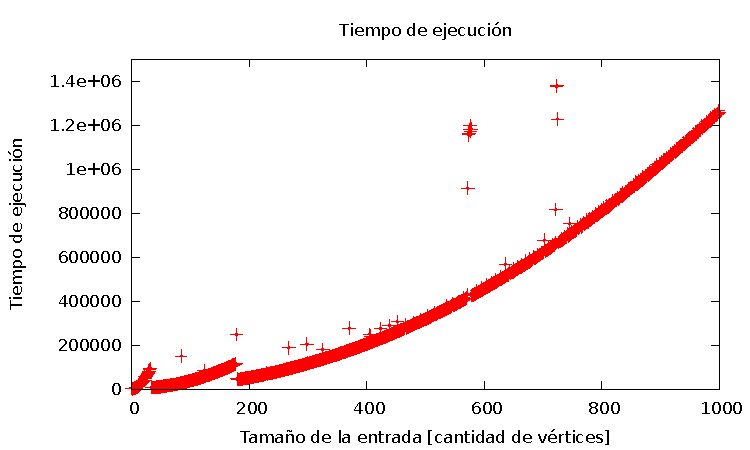
\includegraphics[width=\textwidth]{ej2/cuadratico.pdf}
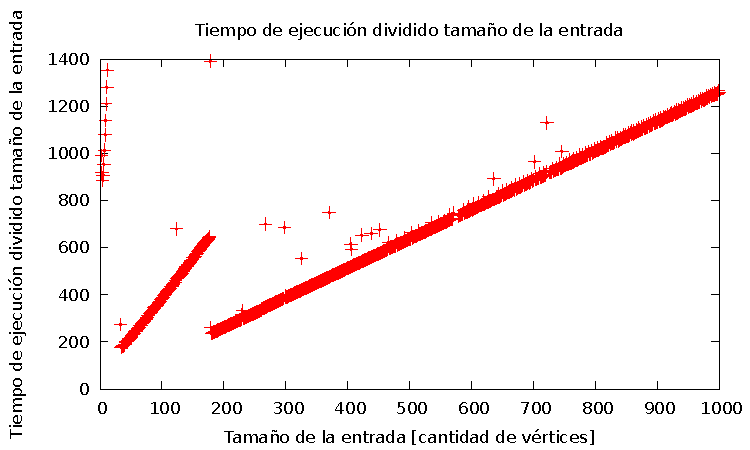
\includegraphics[width=\textwidth]{ej2/lineal.pdf}


\subsection{Compilar y ejecutar}
Desde el directorio src/Ejercicio2:
\begin{itemize}
   \item {\bf Compilar:} ./ej1 make
   \item {\bf Ejecutar:} ./ej1
   \item {\bf Correr casos de test:} ./ej1 tests
   \item {\bf Benchmarks:} ./ej1 bench
\end{itemize}
